\documentclass[12pt, twoside]{fithesis2}

% ===== PACKAGES =====
% language settings
\usepackage[english]{babel}
% enabling new fonts support (nicer)
\usepackage{lmodern}
% setting input encoding
\usepackage[utf8]{inputenc}
% setting output encoding
\usepackage[T1]{fontenc}
% fithesis2 requires csquotes
\usepackage{csquotes}
% set page margins
\usepackage[top=3.0cm, bottom=3.5cm, left=2.9cm, right=1.9cm]{geometry}
% package to make bullet list nicer
\usepackage{enumitem}
% math symbols and environments
\usepackage{mathtools}
\usepackage{amsmath}
\usepackage{amssymb}
% packages for complex tablestj
\usepackage{tabularx}
% package for defining new floating environments
\usepackage{float}
\usepackage[labelfont=]{caption}
% package for drawing
\usepackage{tikz}
\usetikzlibrary{shapes,positioning,fit,plotmarks}
% code listings
\usepackage{listings}
% code highlighting
\usepackage[chapter]{minted}

\usepackage{pdfpages}
\usepackage{afterpage}
\usepackage{dirtree}

% space between paragraphs [smaller space between paragraphs]
\setlength{\parskip}{0.6em plus0.2em minus0.2em}

% bibliography management
\usepackage[
  backend=biber, % use biber
  bibstyle=ieee-alphabetic, %IEEE with alphabetic citations
  citestyle=alphabetic, % citation style
  %citestyle=numeric, % citation style
  url=true, % display urls in bibliography
  hyperref=auto, % detect hyperref and create links
]{biblatex}
\addbibresource{thesis.bib}

% break long urls
\setcounter{biburllcpenalty}{7000}
\setcounter{biburlucpenalty}{8000}

% setting custom colors for links
\usepackage{xcolor}
\definecolor{theme-red}{rgb}{0.62,0.01,0.05}
\definecolor{dark-red}{rgb}{0.6,0.15,0.15}
\definecolor{dark-green}{rgb}{0.15,0.4,0.15}
\definecolor{medium-blue}{rgb}{0,0,0.5}
\definecolor{light-gray}{rgb}{0.93,0.93,0.93}

\def\chapterautorefname{Chapter}

% generating hyperlinks in document
\usepackage{url}
\usepackage{xpatch}
\usepackage[
    plainpages=false, % get the page numbering correctly
    pdfpagelabels, % write arabic labels to all pages
    unicode, % allow unicode characters in links
    colorlinks=true, % use colored links instead of boxed
    linkcolor={theme-red},
    citecolor={theme-red},
    urlcolor={theme-red}
]{hyperref}

\providecommand*{\listingautorefname}{listing}

\newcommand\blankpage{%
    \null
    \thispagestyle{empty}%
    \addtocounter{page}{-1}%
    \newpage}

% ===== FI THESIS SETTINGS =====
\thesistitle{Extracting Parts of Programs into Separate Binaries}
\thesissubtitle{Master's thesis}
\thesisstudent{Tomáš Mészaroš}
\thesiswoman{false}
\thesisfaculty{fi}
\thesisyear{2018}
\thesisadvisor{Mgr. Marek Grác, Ph.D.}
\thesislang{en}

% ===== LATEX DOCUMENT SETTINGS =====
% only put chapters and sections into the TOC
\setcounter{tocdepth}{2}

% renew command for shorter and nicer underscore
\renewcommand{\_}{\leavevmode \kern0.07em\vbox{\hrule width0.4em}}

% ===== COMMANDS =====
% define square symbol
\newcommand{\squarebullet}{\textcolor{black}{\raisebox{0.15em}{\rule{4pt}{4pt}}}}
\newcommand{\emptysquarebullet}{\textcolor{black}{\raisebox{0.10em}{\tiny$\square$}}}

\newenvironment{myItemize}{
  \begin{itemize}[
    leftmargin=2em,
    rightmargin=1em,
    itemsep=\parskip,
    parsep=0em,
    topsep=0em,
    partopsep=0em
]
  \renewcommand{\labelitemi}{\squarebullet}
  \renewcommand{\labelitemii}{\textbullet}
}{
  \end{itemize}
}

\newenvironment{myEnumerate}{
  \begin{enumerate}[
    leftmargin=2em,
    rightmargin=1em,
    itemsep=\parskip,
    parsep=0em,
    topsep=0em,
    partopsep=0em
]
}{
  \end{enumerate}
}

% define new environment for code
\lstnewenvironment{code}{
  \lstset{
  frame=lines,
  rulecolor=\color{black},
  basicstyle=\ttfamily,
  columns=fullflexible,
  showspaces=false,
  showstringspaces=false,
  escapeinside={<*}{*>},
  belowskip=0.2em
  }}{}


% ===== BEGIN DOCUMENT =====
\begin{document}

\FrontMatter
\ThesisTitlePage

% zadanie a prehlasenie
% TODO: Comment this for the electronic version!
%
\includepdf[pages=-]{blank.pdf}
%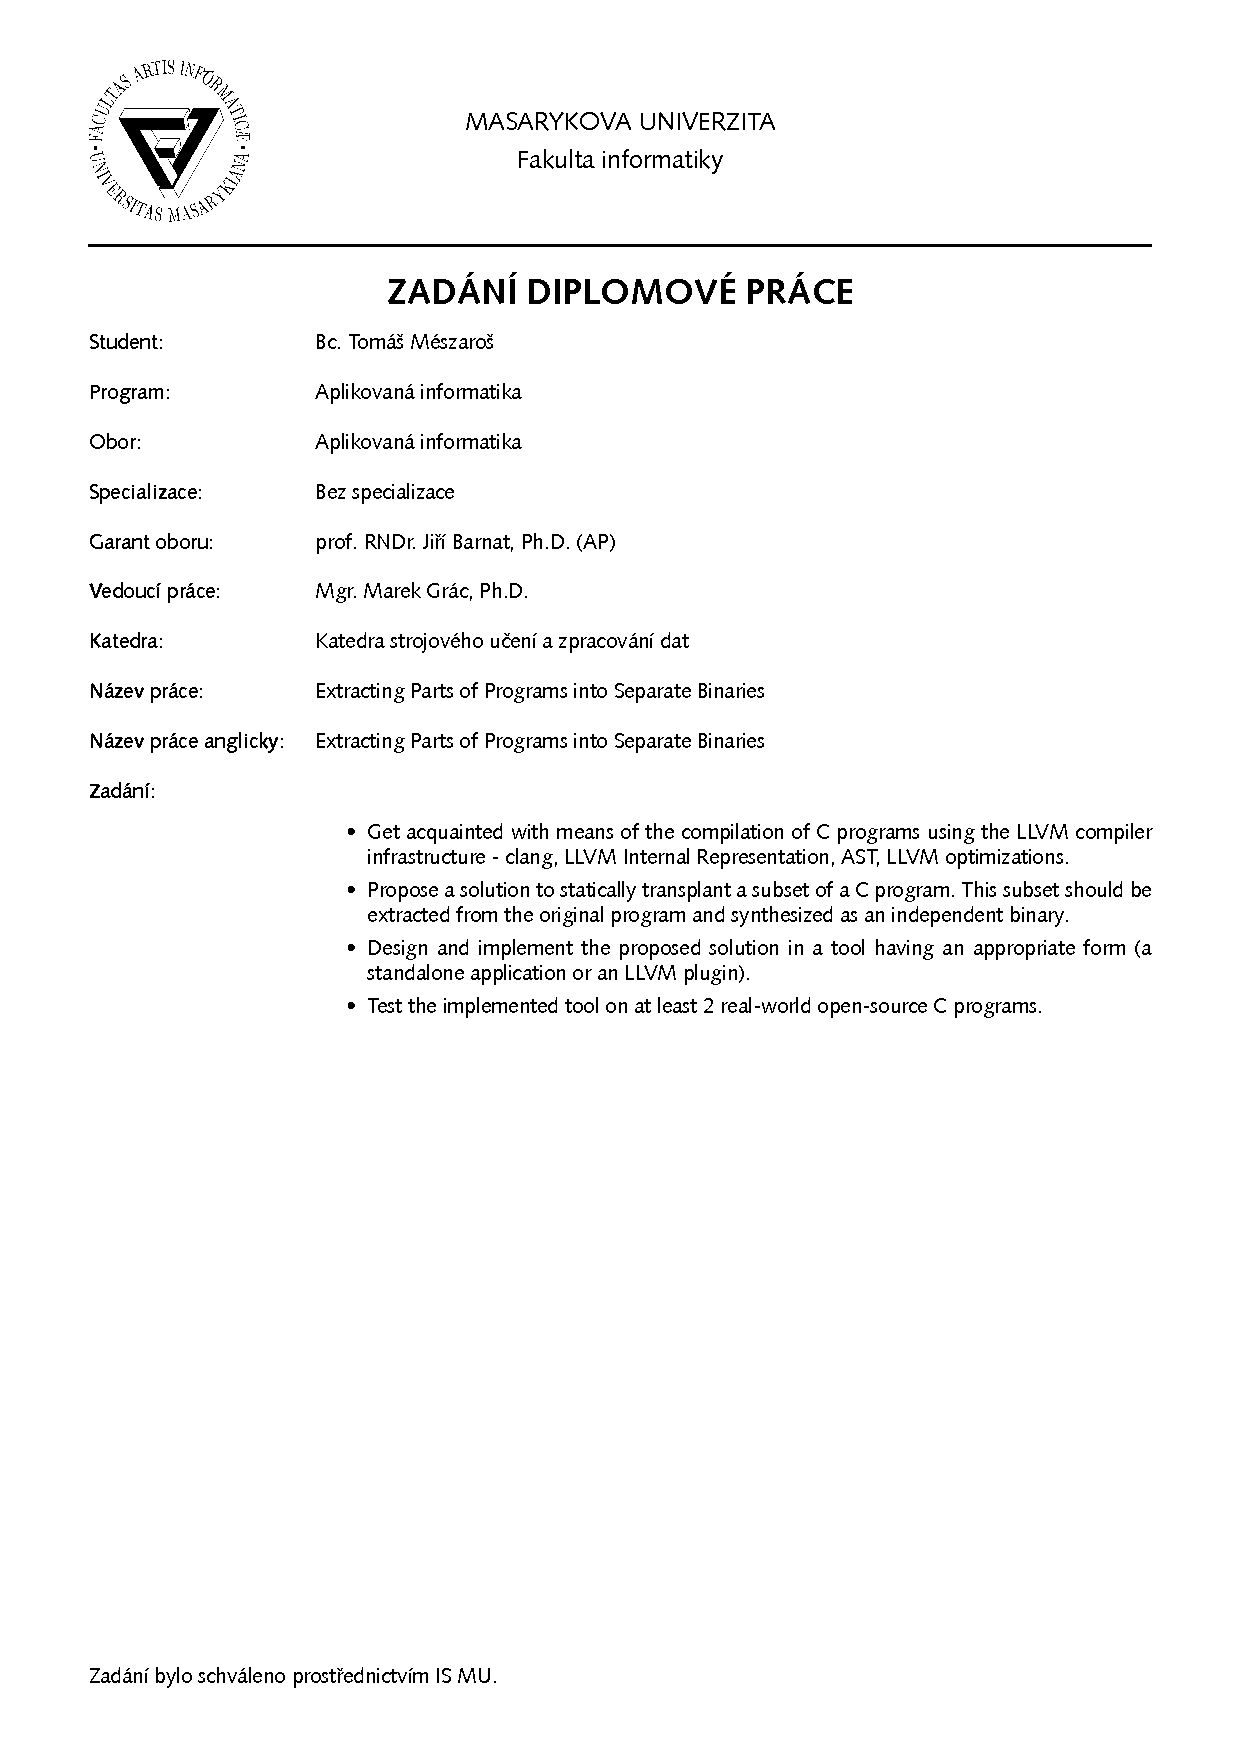
\includepdf[pages=-]{zadanie.pdf}
%
\includepdf[pages=-]{blank.pdf}
%
\includepdf[pages=-]{prehlasenie.pdf}

\begin{ThesisDeclaration}
    \DeclarationText
    \AdvisorName
\end{ThesisDeclaration}

\begin{ThesisThanks}
    Thesis Thanks TBA - Thesis Thanks TBA - Thesis Thanks TBA
    Thesis Thanks TBA - Thesis Thanks TBA - Thesis Thanks TBA
    Thesis Thanks TBA - Thesis Thanks TBA - Thesis Thanks TBA
    Thesis Thanks TBA - Thesis Thanks TBA - Thesis Thanks TBA
    Thesis Thanks TBA - Thesis Thanks TBA - Thesis Thanks TBA
    Thesis Thanks TBA - Thesis Thanks TBA - Thesis Thanks TBA
\end{ThesisThanks}

\begin{ThesisAbstract}
    Thesis Abstract TBA - Thesis Abstract TBA - Thesis Abstract TBA
    Thesis Abstract TBA - Thesis Abstract TBA - Thesis Abstract TBA
    Thesis Abstract TBA - Thesis Abstract TBA - Thesis Abstract TBA
    Thesis Abstract TBA - Thesis Abstract TBA - Thesis Abstract TBA
    Thesis Abstract TBA - Thesis Abstract TBA - Thesis Abstract TBA
    Thesis Abstract TBA - Thesis Abstract TBA - Thesis Abstract TBA
\end{ThesisAbstract}

\begin{ThesisKeyWords}
    keyword, keyword, keyword, keyword, keyword, keyword,
    keyword, keyword, keyword, keyword, keyword, keyword,
    keyword, keyword, keyword, keyword, keyword, keyword
\end{ThesisKeyWords}


\MainMatter
\tableofcontents



% === CHAPTER ==================================================================
\chapter{Introduction}
\label{chap:intro}

TODO: CITATION TEST, REMOVE THIS LATER:

\cite{dg}
\cite{llvm}
\cite{llvm-passes}
\cite{llvm-writing-pass}
\cite{llvm-opt}

User wants to know the value of some variable in the program. He/she can run
debugger of choice, set breakpoint at the selected variable location and let
debugger execute input program step by step until it reaches the selected
variable. Finally, debugger steps on the targeted variable and thus can extract
its value and provide it back to the user.

The procedure described above is usually part of the standard standard approach
when user want to get value of some selected variable during the program
execution. Unfortunately, this approach is cumbersome in case when user want to
execute above procedure many times. Procedure consists of many manual steps
which is time consuming to perform. Ideally, there could be script that takes
line of code (or variable name) as an input and produces output with the value
of the selected target

Normally, this method would require to use debugger with the scripting support
and write scripts that would instruct debugger what exactly to do, basically
replicating the manual approach.

Instead of scripting debugger to do the extraction, we could write tool that
would accept the same user input as the approach above (line of code/variable
name), run analysis on where the execution flow in the program would occur to
get to the target instruction and transplant subset of the input program into
separate binary.

This way, user will have separate, executable that upon running would produce
value of the targeted instruction, without having to manually step thought or
script debugger.

This thesis aims to devise method and implement this method in a tool for
statically transplanting a subset of a C program. Using the devised method, the
selected program subset should be extracted from the original program provided
by the user and synthesized as an independent, executable binary.

Proposed solution should be implemented in a tool having appropriate form,
either as a standalone application or an LLVM plugin. It should easily accept
user to provide their own input programs.

Finally, tool should be used to test at least two real-world open-source C
programs in order to find where the room for improvements is and what could be
improved in the future.


% summary of the thesis

The following sections of this thesis are structured as follows.
In the \autoref{chap:llvm} we will briefly introduce the LLVM compiler
infrastructure.  Explain what makes it so popular and why we picked this tool
for our implementation.
The following \autoref{chap:design}, we will introduce method that is the basis
of this thesis aim.
We will devote \autoref{chap:implementation} for explaining specific details
and intricacies of implementation.
Experiments and their results will be discussed in the chapter
\autoref{chap:experiments}. Finally \autoref{chap:conclusions} summarizes the
results of this thesis and describes possible further research and development
opportunities.


\chapter{The LLVM Compiler Infrastructure}
\label{chap:llvm}

"The LLVM (FOOTNOTE:The name "LLVM" itself is not an acronym; it is the full
name of the project.) Project is a collection of modular and reusable compiler
and toolchain technologies." \cite{llvm}

"an umbrella project that hosts and develops a set of close-knit low-level
toolchain components (e.g., assemblers, compilers, debuggers, etc.), which are
designed to be compatible with existing tools typically used on Unix systems"

"the main thing that sets LLVM apart from other compilers is its internal
architecture." [6] Primary subprojects:

LLVM core clang ...  Strengths: "A major strength of LLVM is its versatility,
flexibility, and reusability"

\section{Intermediate Representation}
\label{sec:llvm-ir}

% subsection
Introduction
- IR AKA LLVM assembly language AKA LLVM

- "LLVM is a Static Single Assignment (SSA) based representation that provides
type safety, low-level operations, flexibility, and the capability of
representing ‘all’ high-level languages cleanly. It is the common code
representation used throughout all phases of the LLVM compilation strategy."

- Aims:
 - "The LLVM representation aims to be light-weight and low-level while being
 expressive, typed, and extensible at the same time."

- Representations of IR:
 - as an in-memory compiler IR
 - as an on-disk bitcode representation (suitable for fast loading by a
 Just-In-Time compiler)
 - as a human readable assembly language representation

% subsection
Example of the IR

We have the following C function add

\begin{minted}[ framesep=2mm,
                autogobble,
                frame=lines]{C}
int add(int a, int b) {
    return a+b;
}
\end{minted}

When using clang compiler with -emit-llvm flag, we get the following representation in IR:

\begin{minted}[ framesep=2mm,
                autogobble,
                frame=lines]{llvm}
define i32 @add(i32 %a, i32 %b) #0 {
entry:
  %a.addr = alloca i32, align 4
  %b.addr = alloca i32, align 4
  store i32 %a, i32* %a.addr, align 4
  store i32 %b, i32* %b.addr, align 4
  %0 = load i32, i32* %a.addr, align 4
  %1 = load i32, i32* %b.addr, align 4
  %add = add nsw i32 %0, %1
  ret i32 %add
\end{minted}

% subsection
High Level Structure

- Module structure:
 - functions
 - global variables
 - symbol table entries

- using LLVM linker for module combination
 - we will use this in practice

- Functions:
 - "A function definition contains a list of basic blocks, forming the CFG
 (Control Flow Graph) for the function."
 - PHI nodes


\section{Optimisations}
\label{sec:llvm-opt}

LLVM uses the concept of Passes for the optimisations. Concrete optimisations
are implemented as Passes that work with some portion of program code (e.g.
Module, Function, Loop, etc.) to collect or transform this portion of the code.
\cite{llvm-passes}

There are the following types of passes:

Analysis passes
- Analysis passes collect information from the IR and feed it into the other
passes. They can be also used for the debugging purposes, for example pass that
counts number of functions in the module.

Examples:

- basiccg: Basic CallGraph Construction
- dot-callgraph: Print Call Graph to “dot” file
- instcount: Counts the various types of Instructions

Transform passes
- Transform passes change the program in some way. They can use some analysis
pass that has been ran before and produced some information.

Examples:

- dce: Dead Code Elimination
- loop-deletion: Delete dead loops
- loop-unroll: Unroll loops

Utility passes
- Utility passes do not fit into analysis passes or transform passes categories.

Examples:

- verify: Module Verifier
- view-cfg: View CFG of function
- instnamer: Assign names to anonymous instructions

\section{Clang}
\label{sec:llvm-clang}

"The Clang project provides a language front-end and tooling infrastructure for
languages in the C language family"

Features and Goals (some overview of clang):
- End-User Features
- Utility and Applications
- Internal Design and Implementation

AST
- what is AST
- AST in clang
- Differences between clang AST and other compilers ASTs
- We will not use clangs AST, we will work directly with IR, it better suits
this project


% === CHAPTER: Design of the Method ============================================
\chapter{Extracting Program Subsets}
\label{chap:design}

% introduction

In this chapter, we will introduce the method for extracting parts of programs
from the provided input. The presented method will not randomly extract program
parts, that would not be useful. Instead, the method determines what parts of
the input program to extract according to the user input. Besides C source code,
user also provides integer value that represents line of code corresponding to
the input C source code. We will call this integer value \textbf{target}.
Our procedure will subsequently calculate possible execution path up to the
target that user provided and extracts this execution path into separate
program.

The whole procedure from the users perspective (including the desired result we
want to achieve) may look like this:

% next point
\begin{myItemize}
\item Lets say the user provided us with the input in the form of the following
C program source code that is stored in the file \mintinline{text}{example.c}:

\begin{minted}[frame=lines, framesep=10pt,linenos]{C}
int foo(int n) {
  int x = n + 10;
  return x;
}

int bar(void) {
   return 42;
}

int main(void) {
  int some_int = 10;
  int foo_result = foo(some_int);
  int bar_result = bar();
  return 0;
}
\end{minted}


Since our method does not work directly with the C source code but instead
works with the LLVM Intermediate Representation (IR), lets use clang and emit
IR from the presented C source code in order to demonstrate our method more
clearly:
\footnote{
Flag \mintinline{text}{-S} tells clang to only run preprocess and
compilation steps, while \mintinline{text}{-emit-llvm} makes sure to use the LLVM
representation for assembler and object files. For detailed description of
various clang flags, visit
\url{https://clang.llvm.org/docs/ClangCommandLineReference.html}.
}

\begin{minted}[frame=lines,framesep=10pt]{bash}
  clang -S -emit-llvm example.c -o example.s
\end{minted}

Emitted LLVM IR is stored in the \mintinline{text}{example.s} and would
have the following contents:
\footnote
{
Strictly speaking, this is not exactly the IR code that would be emmited by the
clang. We have stripped it out of the module info and comments to make it more
readable. To see the unmodified \mintinline{text}{example.s}, please go to the
\autoref{appendix:example}.
}

\begin{minted}[frame=lines,framesep=10pt]{llvm}
define i32 @foo(i32 %n) #0 {
entry:
  %n.addr = alloca i32, align 4
  %x = alloca i32, align 4
  store i32 %n, i32* %n.addr, align 4
  %0 = load i32, i32* %n.addr, align 4
  %add = add nsw i32 %0, 10
  store i32 %add, i32* %x, align 4
  %1 = load i32, i32* %x, align 4
  ret i32 %1
}

define i32 @bar() #0 {
entry:
  ret i32 42
}

define i32 @main() #0 {
entry:
  %retval = alloca i32, align 4
  %some_int = alloca i32, align 4
  %foo_result = alloca i32, align 4
  %bar_result = alloca i32, align 4
  store i32 0, i32* %retval, align 4
  store i32 10, i32* %some_int, align 4
  %0 = load i32, i32* %some_int, align 4
  %call = call i32 @foo(i32 %0)
  store i32 %call, i32* %foo_result, align 4
  %call1 = call i32 @bar()
  store i32 %call1, i32* %bar_result, align 4
  ret i32 0
}
\end{minted}
\end{myItemize}

% next point
\begin{myItemize}
\item User also provided the line number 2 as the target, which corresponds to
the following C code:

\begin{minted}[frame=lines,framesep=10pt]{C}
  int x = n + 10;
\end{minted}

which in turn, corresponds to the following IR:

\begin{minted}[frame=lines,framesep=10pt]{llvm}
  %0 = load i32, i32* %n.addr, align 4
  %add = add nsw i32 %0, 10
  store i32 %add, i32* %x, align 4
\end{minted}

Method for finding mapping between C code and its equivalent IR instructions
will be described in the \autoref{chap:implementation}.
\end{myItemize}

% next point
\begin{myItemize}
\item Now, we can take our method, apply it on the contents of the
\mintinline{text}{example.s} and get the following result:

\begin{minted}[frame=lines,framesep=10pt]{llvm}
define i32 @foo(i32 %n) #0 {
entry:
  %n.addr = alloca i32, align 4
  %x = alloca i32, align 4
  store i32 %n, i32* %n.addr, align 4
  %0 = load i32, i32* %n.addr, align 4
  %add = add nsw i32 %0, 10
  store i32 %add, i32* %x, align 4
  %1 = load i32, i32* %x, align 4
  ret i32 %1
}

define i32 @main() #0 {
entry:
  %some_int = alloca i32, align 4
  %foo_result = alloca i32, align 4
  store i32 10, i32* %some_int, align 4
  %0 = load i32, i32* %some_int, align 4
  %call = call i32 @foo(i32 %0)
  store i32 %call, i32* %foo_result, align 4
  ret i32 0
}
\end{minted}

As we can see, since execution path from the program entry in the
\mintinline{text}{main} function (which we will call \textbf{source}) to the
\textbf{target} does not include function \mintinline{text}{bar} and its
associated instructions, hence they got removed.
\end{myItemize}


\bigskip
% next stuff
Barring implementation specific details (which will be discussed in the
\autoref{chap:implementation}), the method for achieving presented result can be
summarized in the following five steps:

\begin{myEnumerate}
\item Compute data dependencies between instructions.
\item Find connected components in the computed data dependencies inside
every function.
\item Construct call graph, mapping between connected components and functions
they are calling.
\item Find path from source to target in the call graph.
\item Remove functions and connected components that do not depend on the
path.
\end{myEnumerate}

We will describe in detail each step in the remaining sections of the current
chapter.

% === SECTION ===
\section{Computing Data Dependencies}
\label{sec:design-dep}

% motivation
In order to identify what parts of the IR we can afford to remove, it is
imperative to compute dependencies between instructions. We cannot haphazardly
start removing functions left and right because we may remove some instruction
that would be later needed by another instruction.
This unwise action, may in effect produce inconsistent state, which might leave
IR in the unwanted state or even state that would later fail to recompile back
into the executable.

% definitions
We recognize two types of dependencies between IR instructions:

\begin{myItemize}
\item \textbf{Control dependence}. "Control dependence explicitly states what nodes are
controlled by which predicate."
\item \textbf{Data dependence}. "A data dependence edge is between nodes n and m iff n
defines a variable that m uses and there is no intervening definition of that
variable on some path between n and m. In other words, the definitions from n
reach uses in m."
\end{myItemize}

The terminology and algorithms for computing dependencies come from the
master's thesis of Marek Chalupa \textit{Slicing of LLVM Bitcode} \cite{dg}.

% method
The crucial information comes from data dependencies. We need to make sure that
the IR integrity will remain intact after we are done with our transformation.
We have to know which instructions depend which. We cannot afford to remove
blindly any instruction, because it may happen that this removed instruction is
needed by some other instruction.

The above rationale can be demonstrated on the example below:

\begin{minted}[ framesep=2mm,
                autogobble,
                frame=lines]{llvm}
%call3 = call i32 @flag()
store i32 %call3, i32* %f, align 4
%0 = load i32, i32* %f, align 4
\end{minted}

We have tree instructions. We call function flag, capture return value into
variable call3, store value from call3 into variable f and finally load value
from f into 0.

We can see that if we would remove instruction

\begin{minted}[ framesep=2mm,
                autogobble,
                frame=lines]{llvm}
%call3 = call i32 @flag()
\end{minted}

it would mean that call3 is going to be undefined and instruction

\begin{minted}[ framesep=2mm,
                autogobble,
                frame=lines]{llvm}
store i32 %call3, i32* %f, align 4
\end{minted}

would work with undefined variable. This would break integrity of the IR as the
later computation dependent on the

\begin{minted}[ framesep=2mm,
                autogobble,
                frame=lines]{llvm}
store i32 %call3, i32* %f, align 4
\end{minted}

would fail.

We need to make sure we do not corrupt IR with undefined variables.


% === SECTION ===
\section{Finding Connected Components}
\label{sec:design-components}

% References% TODO: put definition of connected component somewhere

Since we know that there are data dependencies between instructions, we can
construct graph G where V is set of vertices (in our case vertex is
instruction) and E is set of edges (in our case, edge between vertices V1 and
V2 represents data dependency between instruction V1 and V2).

Let us demonstrate on the following example. Lets take this simple C function:

\begin{minted}[ framesep=2mm,
                autogobble,
                frame=lines]{C}
int z(void) {
  printf("hello from z\n");
  int tmp = 1;
  return tmp;
}
\end{minted}

Above C code corresponds to the following IR:

\begin{minted}[ framesep=2mm,
                autogobble,
                frame=lines]{llvm}
define i32 @z() #0 {
entry:
  %tmp = alloca i32, align 4
  %call = call i32 (i8*, ...) @printf(i8* ...)
  store i32 1, i32* %tmp, align 4
  %0 = load i32, i32* %tmp, align 4
  ret i32 %0
}
\end{minted}

Graph G would look like (in the adjacency list form):

\begin{minted}[ framesep=2mm,
                autogobble,
                frame=lines]{text}
[%tmp = alloca i32, align 4] -> [store i32 1, i32* %tmp, align 4]
[%call = call i32 (i8*, ...) @printf(i8* ...)] -> []
[store i32 1, i32* %tmp, align 4] -> [%0 = load i32, i32* %tmp, align 4]
[%0 = load i32, i32* %tmp, align 4] -> [ret i32 %0]
[ret i32 %0] -> []
\end{minted}

Now, we can find connected components in G easily by traversing graph using BFS.

\begin{minted}[ framesep=2mm,
                autogobble,
                frame=lines]{text}
FUNCTION: z
- COMPONENT:
    %tmp = alloca i32, align 4
    store i32 1, i32* %tmp, align 4
    %0 = load i32, i32* %tmp, align 4
    ret i32 %0
- COMPONENT:
    %call = call i32 (i8*, ...) @printf(i8* ...)
\end{minted}

Having instructions within function separated into connected components comes
useful. We can see that since call to printf is in the different component than
other instructions. If we were to remove this printf call, integrity of the
instructions in the other component would not be compromised. We can take
advantage of this when we know for sure that we are interested about
instructions in certain components and not in the others. We can proceed and
remove whole components and not compromise integrity.

The procedure describing how are we going to pick components for removal and
remove them will come later.

% === SECTION ===
\section{Constructing Call Graph}
\label{sec:design-callgraph}

% References: some call graph definition

Call graph in general

% citation needed & improve this, add definition of CFG
Call graph is a control flow graph that represents relationship between program
procedures in respect to control flow. Lets have call graph G = {V, E}, where
set of vertices V typically represents functions and set of edges E represents
calls from one function in V to \texttt{another}.

TODO: put here image of stock CFG


Call graph in our case

In our case, call graph represents relationship between individual function
connected components and functions that these components call, more
specifically instruction from component calls.

To demonstrate more clearly what exactly is callgraph in our context, lets take
the following C program:

\begin{minted}[ framesep=2mm,
                autogobble,
                frame=lines]{C}
int y(void) {
  return 2;
}

int x(void) {
  return 1;
}

int main(void) {
  int x_ret = x();
  int y_ret = y();
  return 0;
}
\end{minted}

Classic callgraph would look like:

\begin{minted}[ framesep=2mm,
                autogobble,
                frame=lines]{text}
[main] -> [x, y]
[x] -> []
[y] -> []
\end{minted}

main calls x and y while both x and y do not call anything.

The IR representation of the above program:

\begin{minted}[ framesep=2mm,
                autogobble,
                frame=lines]{llvm}
define i32 @y() #0 {
entry:
  ret i32 2
}

define i32 @x() #0 {
entry:
  ret i32 1
}

define i32 @main() #0 {
entry:
  %retval = alloca i32, align 4
  %x_ret = alloca i32, align 4
  %y_ret = alloca i32, align 4
  store i32 0, i32* %retval, align 4
  %call = call i32 @x()
  store i32 %call, i32* %x_ret, align 4
  %call1 = call i32 @y()
  store i32 %call1, i32* %y_ret, align 4
  ret i32 0
}
\end{minted}

After applying approach from the previous chapter, we get these connected
components:

\begin{minted}[ framesep=2mm,
                autogobble,
                frame=lines]{text}
FUNCTION: y
- COMPONENT: y:1
    ret i32 2

FUNCTION: x
- COMPONENT: x:1
    ret i32 1

FUNCTION: main
- COMPONENT: main:1
    %retval = alloca i32, align 4
    store i32 0, i32* %retval, align 4
- COMPONENT: main:2
    %x_ret = alloca i32, align 4
    %call = call i32 @x()
    store i32 %call, i32* %x_ret, align 4
- COMPONENT: main:3
    %y_ret = alloca i32, align 4
    %call1 = call i32 @y()
    store i32 %call1, i32* %y_ret, align 4
- COMPONENT: main:4
    ret i32 0
\end{minted}

As was written above, call graph in our situation is mapping between individual
components and functions that are being called within these components. That
gives us the following structure:

\begin{minted}[ framesep=2mm,
                autogobble,
                frame=lines]{text}
[y:1] -> []
[x:1] -> []
[main:1] -> []
[main:2] -> [x]
[main:3] -> [y]
[main:4] -> []
\end{minted}

Having call graph represented in the structure above is beneficial for finding
program execution flow path between specific instructions within the program in
relation to their dependencies.

% === SECTION ===
\section{Finding Path from Source to Target}
\label{sec:design-path}

% References: Find some solid def of path, not from wiki, it is lame.
% TODO: some path code/picture example?

from wiki, citation needed dude "In graph theory, a path in a graph is a finite
or infinite sequence of edges which connect a sequence of vertices which, by
most definitions, are all distinct from one another."

In our case, sequence of vertices is sequence of connected components and
sequence of edges which connect these connected components are function calls
(from one component to another component within called function).

The reason why we constructed our special call graph from the connected
components is the following: We want to find path from the source to target and
in doing so, know which connected components are part of this path or not.

Source in our case is entry point to the program, main functions. Target is
supplied by the user and consists of the pair filename, line number. This pair
represents specific instruction (or set of instructions when compiled into IR).

This means that we are finding execution path from main function to the target
fine of code. Potentially, there may exist infinite number of such paths. From
the optimization standpoint, it would be fitting to find all (or at least as
many as we can) paths from source to target and pick some path according to
selected optimization criteria (shortest path, path with smallest connected
components, etc.).

However, for our purposes, it will be sufficient to find any path. We will use
breadth first search to find any path and work with this path in the later
stages (see chapter "removing unneeded stuff").


% === SECTION ===
\section{Removing Dead Instructions and Functions}
\label{sec:design-removing}

% TODO: some stuff in here should be in implementation rationale behind removing stuff & why we need it

The simplest and seemingly correct way would be to remove every connected
component that is not part of the path that we calculated in the earlier
chapter.

This approach would unfortunately produce inconsistent IR. It not enough to
remove only components in the path. We need to include every other component
that is dependent on any other component that is already part of the path.

% subsection
Checking if we have any branching dependent on the @path

- investigating block, collecting basic blocks
 - TBA
- block has no instruction in "if.*" basic block

Then do nothing

- block has some instruction in "if.*" basic block
 - TBA

- Find branch instruction that services this BB and add block associated with this branch instruction to the @path.
 - TBA

% subsection
Computing what dependency blocks we want to keep

- marking every block from @path as to keep
Mark as visited to make sure we do not process this block in BFS.

- setting up initial queue for BFS search
Go over @path and figure out if there are any calls outside the @path. If there
are, put those called blocks for investigation into the @queue.

- running BFS
Run BFS from queue and add everything for keeping that is not visited.

- Collecting everything that we do not want to keep
We store blocks and functions that we want to remove into sets.

% subsection
Removing unwanted blocks

Remove instructions that we stored earier. Watch out for terminators (do not
remove them).

Do not erase instruction that is inside target instructions (We need those
instructions intact.)

% === CHAPTER: Implementation ==================================================
\chapter{Implementation}
\label{chap:implementation}

\cite{llvm-writing-pass}
how do we extract remaining program
adding to the path
removing non-path functions at the end
along with dependencies
before and after code samples
before and after call graphs

% === CHAPTER: Experiments =====================================================
\chapter{Experiments}
\label{chap:experiments}


% === CHAPTER: Conclusions =====================================================
\chapter{Conclusions}
\label{chap:conclusions}

% === SECTION ===
\section{Summary of the Results}
\label{sec:conclusions-summary}

% focus on our specific contributions
% focus on the wider view, what this thesis brought to the world

% === SECTION ===
\section{Further Research and Development}
\label{sec:conclusions-next}

% what could be improved theoretically? (e.g. multiple paths, etc.)
% what could be improved technically? (e.g. better json dump)


% === BIBLIOGRAPHY =============================================================
\appendix

% print complete bibliography
\printbibliography

% === CHAPTER ==================================================================
\chapter{Archive structure}
\label{appendix:archive}

Content of the attached archive:

TBA TBA TBA

% === REMOVE THIS BEFORE PRINTING ==============================================
\chapter{Outline}

Extracting Parts of Programs into Separate Binaries

\begin{myEnumerate}
\item Get acquainted with means of the compilation of C programs using the LLVM
compiler infrastructure - clang, LLVM Internal Representation, AST, LLVM
optimizations.
\item Propose a solution to statically transplant a subset of a C program. This
subset should be extracted from the original program and synthesized as an
independent binary.
\item Design and implement the proposed solution in a tool having an
appropriate form (a standalone application or an LLVM plugin).
\item Test the implemented tool on at least 2 real-world open-source C
programs.
\end{myEnumerate}

\noindent\rule{\textwidth}{1pt}

\begin{myItemize}

\item Introdution
    \begin{myItemize}
    \item Give introduction to wider context
    \item Clearly explain aim of the thesis
    \item Give outline of the following chapters
    \end{myItemize}

\item The LLVM Compiler Infrastructure
    \begin{myItemize}
    \item IR
    \item Optimizations
    \item clang
    \end{myItemize}

\item Extracting Program Subsets
    \begin{myItemize}
    \item Intro
    \item
    \item Computing Data Dependencies
    \item Finding Connected Components
    \item Constructing Call Graph
    \item Finding Path
    \item Removing Unnecessary Parts
    \end{myItemize}

\item Implementation
    \begin{myItemize}
    \item APEX
    \item APEXPass
    \item Input Source Code
    \item Parsing User Input (Locating Target Instructions)
    \item Computing Dependencies using dg
    \item Extracting Target Data (Injecting Exit and Extraction)
        \begin{myItemize}
        \item Stripping debug symbols
        \end{myItemize}
    \end{myItemize}

\item Experiments
    \begin{myItemize}
    \item Experiment 1
    \item Experiment 2
    \item Experiment 3
    \end{myItemize}

\item Conclusion
    \begin{myItemize}
    \item Show our contribution to the problem
    \item Show wider image in context to this thesis
    \end{myItemize}

\end{myItemize}



% === CHAPTER ==================================================================
\chapter{\mintinline{text}{example.s}}
\label{appendix:example}

\begin{minted}[frame=lines, framesep=10pt, breaklines]{llvm}
; ModuleID = 'example.c'
source_filename = "example.c"
target datalayout = "e-m:e-i64:64-f80:128-n8:16:32:64-S128"
target triple = "x86_64-unknown-linux-gnu"

; Function Attrs: noinline nounwind optnone uwtable
define i32 @foo(i32 %n) #0 {
entry:
  %n.addr = alloca i32, align 4
  %x = alloca i32, align 4
  store i32 %n, i32* %n.addr, align 4
  %0 = load i32, i32* %n.addr, align 4
  %add = add nsw i32 %0, 10
  store i32 %add, i32* %x, align 4
  %1 = load i32, i32* %x, align 4
  ret i32 %1
}

; Function Attrs: noinline nounwind optnone uwtable
define i32 @bar() #0 {
entry:
  ret i32 42
}

; Function Attrs: noinline nounwind optnone uwtable
define i32 @main() #0 {
entry:
  %retval = alloca i32, align 4
  %some_int = alloca i32, align 4
  %foo_result = alloca i32, align 4
  %bar_result = alloca i32, align 4
  store i32 0, i32* %retval, align 4
  store i32 10, i32* %some_int, align 4
  %0 = load i32, i32* %some_int, align 4
  %call = call i32 @foo(i32 %0)
  store i32 %call, i32* %foo_result, align 4
  %call1 = call i32 @bar()
  store i32 %call1, i32* %bar_result, align 4
  ret i32 0
}

attributes #0 = { noinline nounwind optnone uwtable "correctly-rounded-divide-sqrt-fp-math"="false" "disable-tail-calls"="false" "less-precise-fpmad"="false" "no-frame-pointer-elim"="true" "no-frame-pointer-elim-non-leaf" "no-infs-fp-math"="false" "no-jump-tables"="false" "no-nans-fp-math"="false" "no-signed-zeros-fp-math"="false" "no-trapping-math"="false" "stack-protector-buffer-size"="8" "target-cpu"="x86-64" "target-features"="+fxsr,+mmx,+sse,+sse2,+x87" "unsafe-fp-math"="false" "use-soft-float"="false" }

!llvm.module.flags = !{!0}
!llvm.ident = !{!1}

!0 = !{i32 1, !"wchar_size", i32 4}
!1 = !{!"clang version 5.0.1 (tags/RELEASE_500/final)"}
\end{minted}

\end{document}
